\paragraph{IUP02 Visualizar datos personales} \hspace{1cm}\\ 
\label{pant:IUP02} 

\textbf{\textcolor[rgb]{0, 0, 0.545098}{Objetivo}}\\
Esta pantalla permite al Practicante visualizar sus datos personales registrados en la herramienta.\\

\textbf{\textcolor[rgb]{0, 0, 0.545098}{Diseño}}\\
En la figura \ref{fig:IUP02} se muestra la pantalla \nameref{fig:IUP02}, por medio de la cual el Practicante visualiza su información personal registrada. \\

En la parte inferior derecha se encuentran los botones Modificar contraseña y Regresar, los cuales corresponden a modificar su contraseña actual o regresar al menú principal.

\begin{figure}[H]
	\centering
		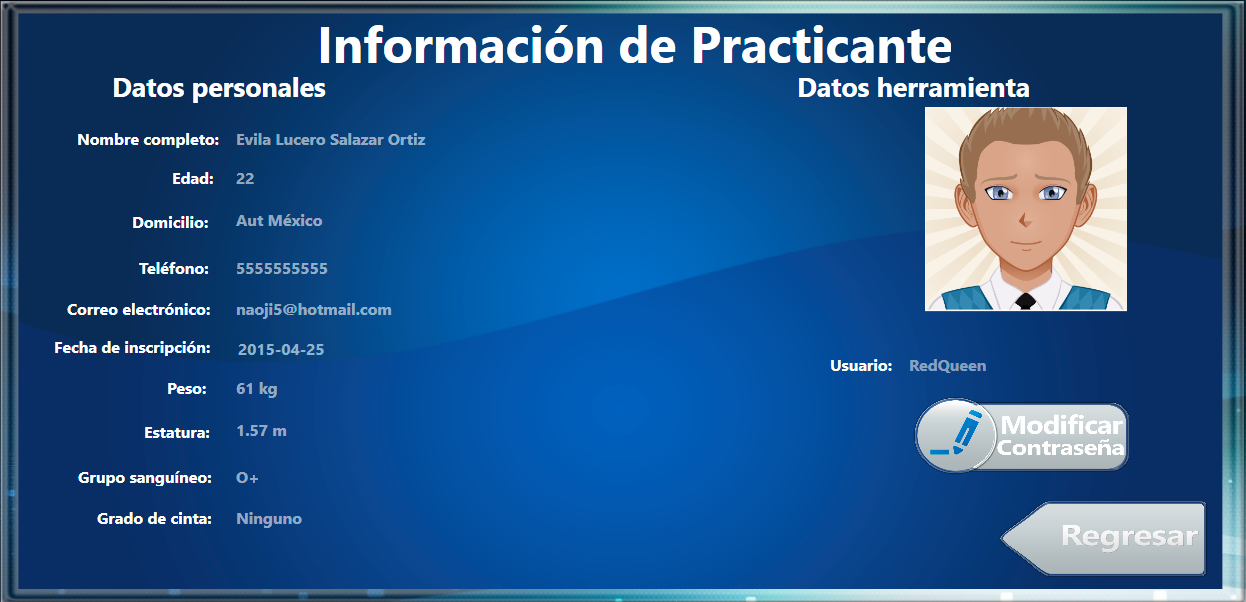
\includegraphics[scale=0.5]{./Figuras/Pantallas/IUP02Visualizar_datos_personales}
	\caption{IUP02 Visualizar datos personales}
	\label{fig:IUP02}
\end{figure}

\textbf{\textcolor[rgb]{0, 0, 0.545098}{Comandos}}
\begin{itemize}
	\item \textbf{\textcolor[rgb]{0, 0, 0.545098}{Modificar contraseña:}} Permite al Practicante modificar su contraseña por medio de la pantalla \nameref{pant:IUP02.1}. \\
	
	\item \textbf{\textcolor[rgb]{0, 0, 0.545098}{Regresar:}} Regresa al menú principal \nameref{menu:MP01}.\\
\end{itemize}

\clearpage